\section{Control}
In the previous section, mathematical modeling of \scp was discussed. In this section, control strategies and their results are shown. Based on models in section \ref{section_modeling}, \anta was controlled to follow desired position, which is a function of time. We will now call this as \Apcnospace.

\subsection{Basic Strategy of \APC}
By assuming that $\ddot{\theta}$ and $\dot{\theta}$ is small enough, we can get correlation between $\theta$ and $T_{1}$, $T_{2}$ as \eqref{simple_assume}.
\begin{equation} \label{simple_assume}
\theta = \frac{c}{2kr}(T_{1}-T_{2})
\end{equation}
By multiplying Laplace transformation of \eqref{thermo-electrical_model} and \eqref{simple_assume}, we can get transfer function of $P$ and $\theta$ as \eqref{apc_transfer}.

\begin{equation} \label{apc_transfer}
\frac{\theta(s)}{P(s)} = \frac{c/2kr}{C_{th}s+\lambda}
\end{equation}

Therefore, process of controlling $\theta$ into $\theta_{ref}$ by applying constant power can be shown as block diagram in Fig.\ref{AntaControl_constant}. 

In this situation, $K_{\theta,P}$ is constant. By applying constant power to only one of the muscle, $\theta$ at steady state was measured. Linear fitting of Fig.\ref{KthetaP} gives us following constant.

\begin{equation}
K_{\theta,P} = \SI{0.185}{\watt\per\degree} \notag
\end{equation}

For fast and precise control, lead compensator was added and feedback, feedforward was applied, as can be seen in Fig.\ref{position_open_loop}, \ref{position_closed_loop}.

\begin{figure}[b]
	\centering
	\begin{minipage}{0.3\textwidth}
		\begin{subfigure}{\linewidth}
			\centering
			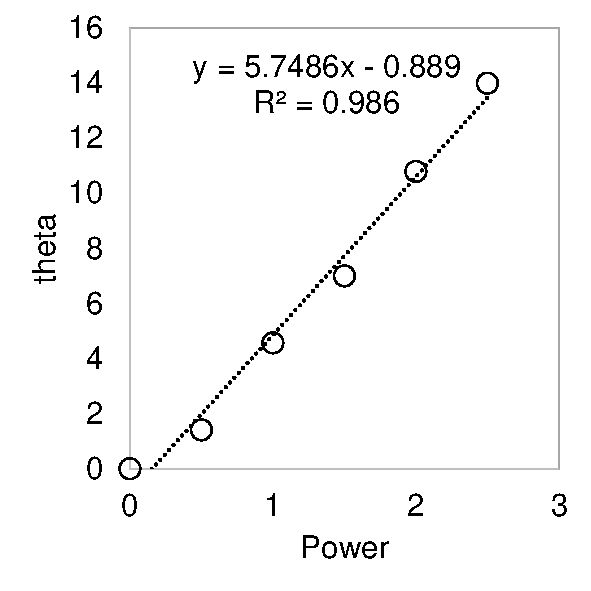
\includegraphics[width=\linewidth]{K_theta_P_v2.pdf}
			\caption{\label{KthetaP}}
		\end{subfigure}
	\end{minipage}%
	\begin{minipage}{0.65\textwidth}
		\begin{subfigure}{\linewidth}
			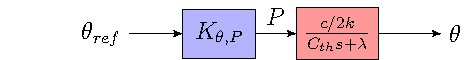
\includegraphics[width=\linewidth]{Diagram(v2)_position_constant_12.pdf}
			\caption{\label{AntaControl_constant}}
		\end{subfigure}
		
		\begin{subfigure}{\linewidth}
			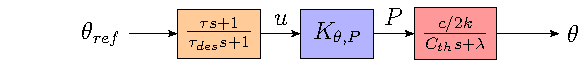
\includegraphics[width=\linewidth]{Diagram(v2)_position_openloop_12.pdf}
			\caption{\label{position_open_loop}}
		\end{subfigure}
		
		\begin{subfigure}{\linewidth}
			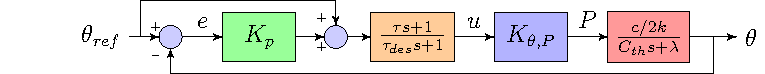
\includegraphics[width=\linewidth]{Diagram(v2)_position_feedback_12.pdf}
			\caption{\label{position_closed_loop}}
		\end{subfigure}
	\end{minipage}
	\caption[Block Diagrams for \APC]{Block diagrams for \apc.\subref{KthetaP} There's a linear relationship between applied power and $\theta$ at steady state.  \subref{AntaControl_constant} Process of obtaining desired angle with constant power \subref{position_open_loop} Process of \apc including lead compensator \subref{position_closed_loop} Process of \apc including feedback and feedforward}
	\label{anta_position_diagrams}
\end{figure}


\subsection{Antagonistic Position Control Strategy for Making Sin Wave Motion}
In this section, we aim to make a simple sin wave motion of \anta like \eqref{theta_ref}. By doing this, we could check the possibility of \apc for any complicated motion. Basically, according to the equation \eqref{simple_assume}, we can increase $\theta$ by heating muscle 1 and decrease $\theta$ by heating muscle 2. 
By assuming that $\ddot{\theta}$ and $\dot{\theta}$ is small enough, \eqref{EqAnta} can be approximated into \eqref{EqAngleTempDiff}.

\begin{equation}\label{EqAngleTempDiff}
\theta=\frac{c}{2kr}(T_1-T_2)
\end{equation}

Therefore, we used a strategy shown in Table.\ref{table_apc_basic}

\begin{equation}\label{theta_ref}
\theta_{ref}(t)=(\SI{9}{\degree})\sin(2\pi 0.025t)
\end{equation}

\begin{table}[h]
	\caption{Basic strategy of \apc for making sin wave motion.}
	\label{table_apc_basic}
	\begin{center}
		\begin{tabular}{c||c|c|c|c}
			\hline
			Time(s) & 0-10 & 10-20 & 20-30 & 30-40 \\
			\hline
			Muscle 1 & Heat & Keep & Keep & Heat \\
			Muscle 2 & Keep & Heat & Heat & Keep \\
			\hline
			$\theta$ & increase & decrease & decrease & increase \\
			\hline
		\end{tabular}
	\end{center}
\end{table}

Since the Laplace transformation of \eqref{theta_ref} is too complicated, we used an approximation shown in \eqref{theta_ref_approx} by dividing \eqref{theta_ref} into 12 steps. In this case, demanded power can be calculated as \eqref{power_derived}. ($n=12$)
\footnote{In equation \eqref{power_derived}, $\theta_{ref,pre}$ is value of $\theta_{ref}$ in previous step. Also, $t$ is elapsed time after starting new step.}
\begin{equation} \label{theta_ref_approx}
% \begin{aligned} 
\theta_{ref}(t) = \sum_{i=0}^{n-1}{(\theta_{ref,i+1}-\theta_{ref,i})U(t-i\Delta T)} 
% \theta_{ref}(t) & = \sum_{i=0}^{n-1}{(\theta_{ref,i+1}-\theta_{ref,i})U(t-i\Delta T)} \\
% & = \sum_{i=0}^{n-1}{(\sin{\frac{2(i+1)\pi}{n}}-\sin{\frac{2i\pi}{n}})U(t-40\frac{i}{n})} \\
% \end{aligned}
\end{equation}

\begin{equation} \label{power_derived}
P(t)=\theta_{ref}K_{\theta,P}(1+(\frac{\theta_{ref}-\theta_{ref,pre}}{\theta_{ref}})(\frac{\tau}{\tau_{des}}-1)e^{-\frac{t}{\tau_{des}}})
\end{equation}

 %Through these steps, we can do \apc as a sin wave form.

\begin{figure}[t]
	\centering
	\begin{subfigure}[t]{0.46\textwidth}
		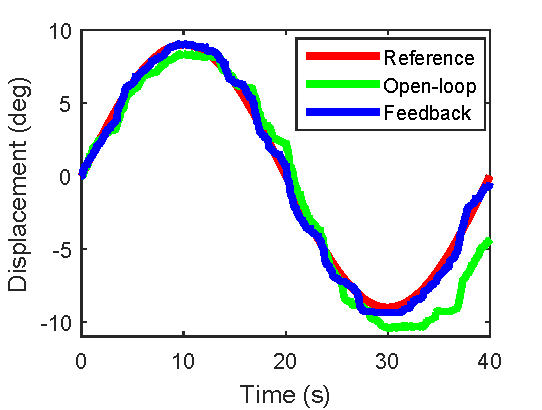
\includegraphics[width=\textwidth]{SinWave.pdf}
		\caption{\label{positionControl_sin}}
	\end{subfigure}%
	\begin{subfigure}[t]{0.46\textwidth}
		\includegraphics[width=\textwidth]{example-image-c}
		\caption{\label{positionControl_sin_power}}
	\end{subfigure}
	\caption[\APC by only heating]{\APC by only heating. \subref{positionControl_sin} Measured arm's angular position in function of time. Feedback control had smaller error than open-loop control. \subref{positionControl_sin_power} Used power of each \scpnospace s(Open loop)}
	\label{positionControl}
\end{figure}



\clearpage



\subsection{Sustainable Antagonistic Position Control Strategy with cooling method}\label{section_simulation}
In previous section, the method for making sin wave motion was discussed. But since the temperature of muscle in initial state and final state is significantly different, it won't be sustainable because the temperature will keep going up. Therefore, we need to make the temperature of initial state and final state to be same. This can be done by cooling the muscle during last 1/4 period of sin wave, as shown in table \ref{table_apc_sustain}.

\begin{table}[b]
	\caption{Sustainable \Apc strategy by using cooling}
	\label{table_apc_sustain}
	\begin{center}
		\begin{tabular}{c||c|c|c|c|c|c}
			\hline
			Time(s) & 0 & 0-10 & 10-20 & 20-30 & 30-40 & 40 \\
			\hline
			Muscle 1 & $T_0$ & Heat & Keep & Keep & Weakly Cool & $T_0$ \\
			Muscle 2 & $T_0$ & Keep & Heat & Heat & Strongly Cool & $T_0$ \\
			\hline
			$\theta$ & $0^{\circ}$ & increase & decrease & decrease & increase & $0^{\circ}$ \\
			\hline
		\end{tabular}
	\end{center}
\end{table}

\subsubsection{Demonstration}
First, we demonstrated open-loop control of cooling speed. Two-period sin wave control was done, and cooling was done in during $t=$\SI{40}{\second} - \SI{50}{\second}\footnote{This slightly differs from table \ref{table_apc_sustain}.}. In order to cool as much as possible, muscle 2 was cooled for all time, and muscle 1 was `weakly' cooled by repeatedly opening and closing the solenoid valve. As a result, we got an rms error 26.6\% for open-loop control, and 6.7\% for closed-loop control.(Fig.\ref{sustain_demo})

%After the demonstration, we concluded that an appropriate time for cooling will be \SI{30}{\second}-\SI{40}{\second}, not \SI{40}{\second} - \SI{50}{\second}. It is because 
\begin{figure}[t]
	\centering
	\begin{subfigure}[t]{0.47\textwidth}
		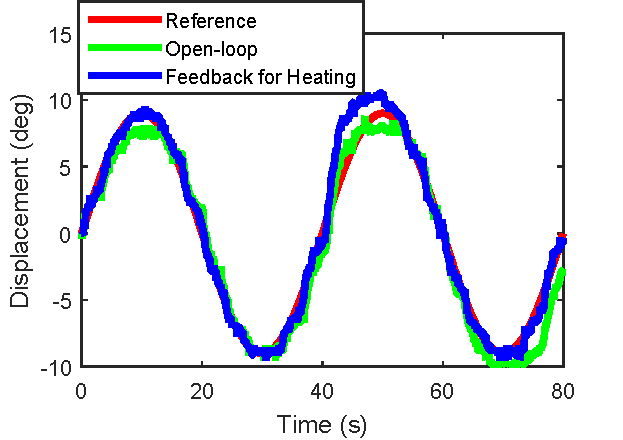
\includegraphics[width=\textwidth]{SinWave_cooling.pdf}
		\caption{\label{SinWave_cooling}}
	\end{subfigure}
	~
	\begin{subfigure}[t]{0.46\textwidth}
		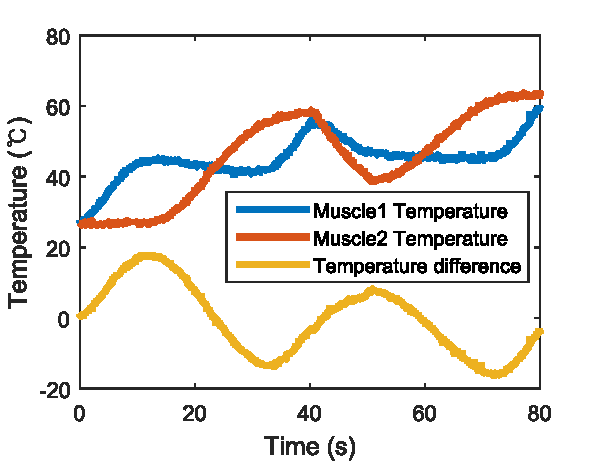
\includegraphics[width=\textwidth]{SinWaveC_T.pdf}
		\caption{\label{Sinwave_C_T}}
	\end{subfigure}
	\caption[Sustainable Open-Loop \APC Demonstration]{Sustainable open-loop \apc demonstration. \subref{SinWave_cooling} Arm's angle in function of time. \subref{Sinwave_C_T} Temperature of two muscles in function of time. We checked that sustainable \apc is possible by cooling for some time.}
	\label{sustain_demo}
\end{figure}

\subsubsection{Simulation}


Integrating \eqref{dynamic_calculation_tau} and \eqref{lambda_control}, we can get \eqref{tau_modification}.
\begin{equation} \label{tau_modification} 
\begin{aligned} 
\tau & = \frac{C_{th}}{\lambda} \\
& = \frac{1.81}{0.77\cdot r + 0.10} \\ 
\end{aligned}
\end{equation}

Also, time derivative of \eqref{simple_assume} and \eqref{theta_ref}, we can get \eqref{theta_diff} where $t$ is time elapsed since $t=\SI{30}{\second}$.

\begin{equation} \label{theta_diff}
\begin{aligned} 
\frac{d\theta}{dt} & = \frac{c}{2kr}\cdot\frac{d}{dt}(T_{1}-T_{2}) \\
& = 9^{\circ}(2\pi\cdot 0.025)\sin{2\pi\cdot 0.025t} 
\end{aligned}
\end{equation}


What we have to do is decreasing $(T_{1}+T_{2})/2$, so we will use following equation with carefully chosen constant $\alpha = 0.23$. 
\begin{equation}
\frac{d}{dt}(T_{1}+T_{2}) = -\alpha(T_{1}+T_{2}-2T_{ambient}) \notag
\end{equation}

Therefore, by using \eqref{thermo-electrical_model} for each muscles, we can calculate needed $\lambda_{1}$, $\lambda_{2}$. The block diagram which represents feedback control of thermal conductivities is shown in Fig.\ref{diagram_sustainable}.

\begin{figure}[t]
	\centering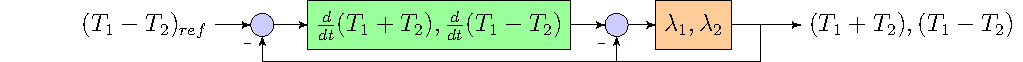
\includegraphics[width=\textwidth]{Diagram_sustainable.pdf}
	\caption{Block diagram for sustainable \apcnospace.}
	\label{diagram_sustainable}
\end{figure}

To make sustainable \apc possible, $\lambda$ must be between $\SI{0.25}{\watt\per\degreeCelsius}$ and $\SI{0.60}{\watt\per\degreeCelsius}$ for all time. Therefore, possibility of this control strategy was verified by thermal simulation.
%We can guess that $\lambda_{1}$ have to decrease and $\lambda_{2}$ have to increase. 

The limit of thermal conductivity is $0.25<\lambda<0.6$, according to \eqref{lambda_control}. In time interval \SI{30}{\second} - \SI{40}{\second}, $\lambda_{1}$ have to decrease and $\lambda_{2}$ have to increase. Therefore, we need to make $\lambda_{1}$ and $\lambda_{2}$ to reach its limit as late as possible. This is determined by constant $\alpha$. 
In Fig.\ref{Sinwave_C_T}, we could observe that two of the muscles' average temperature has increased approximately  \SI{30}{\degreeCelsius}. This means that we have to cool down the average temperature at least \SI{30}{\degreeCelsius}. 

Simulation was carefully done by applying \eqref{thermo-electrical_model} and \eqref{EqAnta}, using the constants we got in section \ref{section_modeling}. The differential equation was numerically solved with 4th Runge-Kutta method.

\begin{figure}[t]
	\centering
	\begin{subfigure}[t]{0.45\textwidth}
		\centering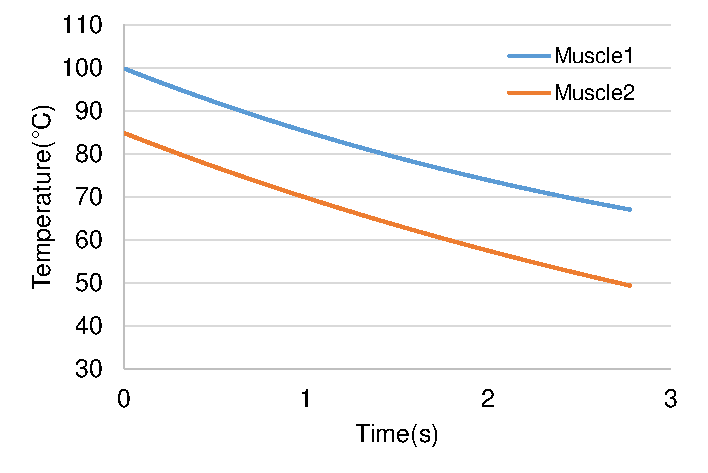
\includegraphics[width=\textwidth]{cool_control_T.pdf}
		\caption{\label{cool_control_T}}
	\end{subfigure}%
	\begin{subfigure}[t]{0.45\textwidth}
		\centering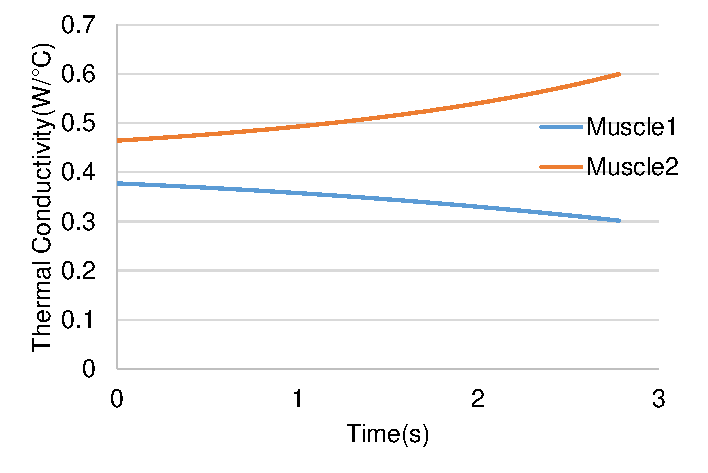
\includegraphics[width=\textwidth]{cool_control_lambda.pdf}
		\caption{\label{cool_control_lambda}}
	\end{subfigure}
	\caption[Sustainable Closed-Loop \APC Simulation]{\subref{cool_control_T} Temperature of two muscles in function of time after $t=\SI{30}{\second}$. \subref{cool_control_lambda} Thermal conductivity of two muscles in function of time. }
	\label{cool_simulation}
\end{figure}

Through some times of simulations, we had concluded that $\alpha = 0.23$ is the best. The result of simulation with this value is shown in Fig.\ref{cool_simulation}. In Fig.\ref{cool_control_T}, we can observe that average temperature of two muscles had decreased over \SI{30}{\degreeCelsius}, before reaching limit thermal conductivity as shown in Fig.\ref{cool_control_lambda}. Therefore, we can conclude that feedback cooling control is possible.


